% Options for packages loaded elsewhere
\PassOptionsToPackage{unicode}{hyperref}
\PassOptionsToPackage{hyphens}{url}
% !TeX program = pdfLaTeX
\documentclass[12pt]{article}
\usepackage{amsmath}
\usepackage{graphicx,psfrag,epsf}
\usepackage{enumerate}
\usepackage[]{natbib}
\usepackage{textcomp}


%\pdfminorversion=4
% NOTE: To produce blinded version, replace "0" with "1" below.
\newcommand{\blind}{0}

% DON'T change margins - should be 1 inch all around.
\addtolength{\oddsidemargin}{-.5in}%
\addtolength{\evensidemargin}{-1in}%
\addtolength{\textwidth}{1in}%
\addtolength{\textheight}{1.7in}%
\addtolength{\topmargin}{-1in}%

%% load any required packages here


% Pandoc syntax highlighting
\usepackage{color}
\usepackage{fancyvrb}
\newcommand{\VerbBar}{|}
\newcommand{\VERB}{\Verb[commandchars=\\\{\}]}
\DefineVerbatimEnvironment{Highlighting}{Verbatim}{commandchars=\\\{\}}
% Add ',fontsize=\small' for more characters per line
\usepackage{framed}
\definecolor{shadecolor}{RGB}{248,248,248}
\newenvironment{Shaded}{\begin{snugshade}}{\end{snugshade}}
\newcommand{\AlertTok}[1]{\textcolor[rgb]{0.94,0.16,0.16}{#1}}
\newcommand{\AnnotationTok}[1]{\textcolor[rgb]{0.56,0.35,0.01}{\textbf{\textit{#1}}}}
\newcommand{\AttributeTok}[1]{\textcolor[rgb]{0.13,0.29,0.53}{#1}}
\newcommand{\BaseNTok}[1]{\textcolor[rgb]{0.00,0.00,0.81}{#1}}
\newcommand{\BuiltInTok}[1]{#1}
\newcommand{\CharTok}[1]{\textcolor[rgb]{0.31,0.60,0.02}{#1}}
\newcommand{\CommentTok}[1]{\textcolor[rgb]{0.56,0.35,0.01}{\textit{#1}}}
\newcommand{\CommentVarTok}[1]{\textcolor[rgb]{0.56,0.35,0.01}{\textbf{\textit{#1}}}}
\newcommand{\ConstantTok}[1]{\textcolor[rgb]{0.56,0.35,0.01}{#1}}
\newcommand{\ControlFlowTok}[1]{\textcolor[rgb]{0.13,0.29,0.53}{\textbf{#1}}}
\newcommand{\DataTypeTok}[1]{\textcolor[rgb]{0.13,0.29,0.53}{#1}}
\newcommand{\DecValTok}[1]{\textcolor[rgb]{0.00,0.00,0.81}{#1}}
\newcommand{\DocumentationTok}[1]{\textcolor[rgb]{0.56,0.35,0.01}{\textbf{\textit{#1}}}}
\newcommand{\ErrorTok}[1]{\textcolor[rgb]{0.64,0.00,0.00}{\textbf{#1}}}
\newcommand{\ExtensionTok}[1]{#1}
\newcommand{\FloatTok}[1]{\textcolor[rgb]{0.00,0.00,0.81}{#1}}
\newcommand{\FunctionTok}[1]{\textcolor[rgb]{0.13,0.29,0.53}{\textbf{#1}}}
\newcommand{\ImportTok}[1]{#1}
\newcommand{\InformationTok}[1]{\textcolor[rgb]{0.56,0.35,0.01}{\textbf{\textit{#1}}}}
\newcommand{\KeywordTok}[1]{\textcolor[rgb]{0.13,0.29,0.53}{\textbf{#1}}}
\newcommand{\NormalTok}[1]{#1}
\newcommand{\OperatorTok}[1]{\textcolor[rgb]{0.81,0.36,0.00}{\textbf{#1}}}
\newcommand{\OtherTok}[1]{\textcolor[rgb]{0.56,0.35,0.01}{#1}}
\newcommand{\PreprocessorTok}[1]{\textcolor[rgb]{0.56,0.35,0.01}{\textit{#1}}}
\newcommand{\RegionMarkerTok}[1]{#1}
\newcommand{\SpecialCharTok}[1]{\textcolor[rgb]{0.81,0.36,0.00}{\textbf{#1}}}
\newcommand{\SpecialStringTok}[1]{\textcolor[rgb]{0.31,0.60,0.02}{#1}}
\newcommand{\StringTok}[1]{\textcolor[rgb]{0.31,0.60,0.02}{#1}}
\newcommand{\VariableTok}[1]{\textcolor[rgb]{0.00,0.00,0.00}{#1}}
\newcommand{\VerbatimStringTok}[1]{\textcolor[rgb]{0.31,0.60,0.02}{#1}}
\newcommand{\WarningTok}[1]{\textcolor[rgb]{0.56,0.35,0.01}{\textbf{\textit{#1}}}}

% tightlist command for lists without linebreak
\providecommand{\tightlist}{%
  \setlength{\itemsep}{0pt}\setlength{\parskip}{0pt}}



\usepackage{booktabs}
\usepackage{longtable}
\usepackage{array}
\usepackage{multirow}
\usepackage{wrapfig}
\usepackage{float}
\usepackage{colortbl}
\usepackage{pdflscape}
\usepackage{tabu}
\usepackage{threeparttable}
\usepackage{threeparttablex}
\usepackage[normalem]{ulem}
\usepackage{makecell}
\usepackage{xcolor}

\IfFileExists{bookmark.sty}{\usepackage{bookmark}}{\usepackage{hyperref}}
\IfFileExists{xurl.sty}{\usepackage{xurl}}{} % add URL line breaks if available
\hypersetup{
  pdftitle={Title here},
  pdfkeywords={3 to 6 keywords, that do not appear in the title},
  hidelinks,
  pdfcreator={LaTeX via pandoc}}



\begin{document}


\def\spacingset#1{\renewcommand{\baselinestretch}%
{#1}\small\normalsize} \spacingset{1}


%%%%%%%%%%%%%%%%%%%%%%%%%%%%%%%%%%%%%%%%%%%%%%%%%%%%%%%%%%%%%%%%%%%%%%%%%%%%%%

\if0\blind
{
  \title{\bf Title here}

  \author{
        Cassandra Jin \thanks{The authors gratefully acknowledge
\ldots{}} \\
    Department of Mathematics and Statistics, Amherst College\\
      }
  \maketitle
} \fi

\if1\blind
{
  \bigskip
  \bigskip
  \bigskip
  \begin{center}
    {\LARGE\bf Title here}
  \end{center}
  \medskip
} \fi

\bigskip
\begin{abstract}
The text of your abstract. 200 or fewer words. It is intended to provide
an overview of your paper and may be similar to your synopsis. Note that
an abstract can only include one paragraph in this format. You may want
to put your synopsis here as you work to refer to it easily.
\end{abstract}

\noindent%
{\it Keywords:} 3 to 6 keywords, that do not appear in the title

\vfill

\newpage
\spacingset{1.9} % DON'T change the spacing!

\hypertarget{introduction}{%
\section{Introduction}\label{introduction}}

This template will be used for you to submit your final project. You'll
need to install the \emph{rticles} package, make sure you have the
agsm.bst file and bibliography.bib file, and the gfx folder and figure
file in order to compile. If you make your own bibliography.bib file
later, that's fine - change the name above to match your file name.
You'll want the setup for the file to look the same in your repo as in
the class repo, and then compile to asa\_article when you knit. You
should change the name of the file to something other than ``test''
though. Remember that if something goes wrong with the file, you can
always look back at the class repo for the original files and their
structure.

This template was adapted from the template Prof.~Horton provided Stat
495 in Fall 2021, used with permission.

\hypertarget{more-on-the-template}{%
\section{More on the template}\label{more-on-the-template}}

\label{sec:template}

This template demonstrates some of the basic LaTeX commands and syntax
you'll need to know to use the \texttt{rticles} package to generate a
readable report using R Markdown. Markdown allows various formatting and
you can find formatting cheatsheets or guides online to assist as well.
Here's an example with bullets and some advice:

\begin{itemize}
\tightlist
\item
  I would encourage you to look closely at this file and explore the
  various parts and pieces.
\item
  I would suggest that you format your Rmd file so that you have only
  one sentence per line.
\item
  It makes it \emph{much} easier to see changes in your GitHub commits.
\end{itemize}

\section{Verifications}
\label{sec:verify}

This section will be just long enough to illustrate what a full page of
text looks like, for margins and spacing.

Note that we can refer to sections (e.g., this is section
\ref{sec:verify}, while the previous section was section
\ref{sec:template}).

Note that we should refer to work using the BibTeX system. Here we can
reference papers by \citet{Campbell02} and \citet{Schubert13} through
inline citations (see the \texttt{bibliography.bib} file for the
reference database).

More work that is relevant can also be cited in a traditional fashion
\citep[\citet{Galyardt14mmm},\citet{Galyardt12dis}]{Chi81}.

Note that you can capitalize proper nouns in citations
\citep{Campbell02} (again, see \texttt{bibliography.bib}).

We also test some other ways to do the citations, such as \cite{Chi81},
and \citep{Campbell02}. These both work. The latter puts the citation in
parentheses. You can also use \citet{Chi81}, though this seems to have
similar behavior to just cite.

The quick brown fox jumped over the lazy dog. The quick brown fox jumped
over the lazy dog. The quick brown fox jumped over the lazy dog. The
quick brown fox jumped over the lazy dog. \textbf{With this spacing we
have 30 lines per page.}

The quick brown fox jumped over the lazy dog. The quick brown fox jumped
over the lazy dog. The quick brown fox jumped over the lazy dog. The
quick brown fox jumped over the lazy dog. The quick brown fox jumped
over the lazy dog.

The quick brown fox jumped over the lazy dog. The quick brown fox jumped
over the lazy dog. The quick brown fox jumped over the lazy dog. The
quick brown fox jumped over the lazy dog. The quick brown fox jumped
over the lazy dog. The quick brown fox jumped over the lazy dog. The
quick brown fox jumped over the lazy dog. The quick brown fox jumped
over the lazy dog. The quick brown fox jumped over the lazy dog. The
quick brown fox jumped over the lazy dog.

The quick brown fox jumped over the lazy dog. The quick brown fox jumped
over the lazy dog. The quick brown fox jumped over the lazy dog. The
quick brown fox jumped over the lazy dog. The quick brown fox jumped
over the lazy dog. The quick brown fox jumped over the lazy dog. The
quick brown fox jumped over the lazy dog. The quick brown fox jumped
over the lazy dog. The quick brown fox jumped over the lazy dog. The
quick brown fox jumped over the lazy dog.

The quick brown fox jumped over the lazy dog. The quick brown fox jumped
over the lazy dog. The quick brown fox jumped over the lazy dog. The
quick brown fox jumped over the lazy dog. The quick brown fox jumped
over the lazy dog. The quick brown fox jumped over the lazy dog. The
quick brown fox jumped over the lazy dog. The quick brown fox jumped
over the lazy dog. The quick brown fox jumped over the lazy dog. The
quick brown fox jumped over the lazy dog.

The quick brown fox jumped over the lazy dog. The quick brown fox jumped
over the lazy dog. The quick brown fox jumped over the lazy dog. The
quick brown fox jumped over the lazy dog. The quick brown fox jumped
over the lazy dog. The quick brown fox jumped over the lazy dog. The
quick brown fox jumped over the lazy dog. The quick brown fox jumped
over the lazy dog. The quick brown fox jumped over the lazy dog. The
quick brown fox jumped over the lazy dog.

The quick brown fox jumped over the lazy dog. The quick brown fox jumped
over the lazy dog. The quick brown fox jumped over the lazy dog. The
quick brown fox jumped over the lazy dog. The quick brown fox jumped
over the lazy dog. The quick brown fox jumped over the lazy dog. The
quick brown fox jumped over the lazy dog. The quick brown fox jumped
over the lazy dog. The quick brown fox jumped over the lazy dog. The
quick brown fox jumped over the lazy dog.

The quick brown fox jumped over the lazy dog. The quick brown fox jumped
over the lazy dog. The quick brown fox jumped over the lazy dog. The
quick brown fox jumped over the lazy dog. The quick brown fox jumped
over the lazy dog. The quick brown fox jumped over the lazy dog. The
quick brown fox jumped over the lazy dog. The quick brown fox jumped
over the lazy dog. The quick brown fox jumped over the lazy dog. The
quick brown fox jumped over the lazy dog.

The quick brown fox jumped over the lazy dog. The quick brown fox jumped
over the lazy dog. The quick brown fox jumped over the lazy dog. The
quick brown fox jumped over the lazy dog. The quick brown fox jumped
over the lazy dog. The quick brown fox jumped over the lazy dog. The
quick brown fox jumped over the lazy dog. The quick brown fox jumped
over the lazy dog. The quick brown fox jumped over the lazy dog. The
quick brown fox jumped over the lazy dog.

The quick brown fox jumped over the lazy dog. The quick brown fox jumped
over the lazy dog. The quick brown fox jumped over the lazy dog. The
quick brown fox jumped over the lazy dog. The quick brown fox jumped
over the lazy dog. The quick brown fox jumped over the lazy dog. The
quick brown fox jumped over the lazy dog. The quick brown fox jumped
over the lazy dog. The quick brown fox jumped over the lazy dog. The
quick brown fox jumped over the lazy dog.

\hypertarget{examples}{%
\section{Examples}\label{examples}}

Lots of things can be done in this template.

\begin{Shaded}
\begin{Highlighting}[]
\NormalTok{iris }\SpecialCharTok{\%\textgreater{}\%}
  \FunctionTok{group\_by}\NormalTok{(Species) }\SpecialCharTok{\%\textgreater{}\%}
  \FunctionTok{summarize}\NormalTok{(}\AttributeTok{count =} \FunctionTok{n}\NormalTok{()) }\SpecialCharTok{\%\textgreater{}\%}
\NormalTok{  knitr}\SpecialCharTok{::}\FunctionTok{kable}\NormalTok{(}
    \AttributeTok{caption =} \StringTok{"This is a sample table caption that should interpret the table!"}\NormalTok{)}
\end{Highlighting}
\end{Shaded}

\begin{table}

\caption{\label{tab:sample-table1}This is a sample table caption that should interpret the table!}
\centering
\begin{tabular}[t]{l|r}
\hline
Species & count\\
\hline
setosa & 50\\
\hline
versicolor & 50\\
\hline
virginica & 50\\
\hline
\end{tabular}
\end{table}

Table \ref{tab:sample-table1} displays the number of irises per species.

\begin{Shaded}
\begin{Highlighting}[]
\NormalTok{iris }\SpecialCharTok{\%\textgreater{}\%} 
  \FunctionTok{ggplot}\NormalTok{(}\FunctionTok{aes}\NormalTok{(}\AttributeTok{y =}\NormalTok{ Sepal.Width, }\AttributeTok{color =}\NormalTok{ Species)) }\SpecialCharTok{+}
  \FunctionTok{geom\_boxplot}\NormalTok{()}
\end{Highlighting}
\end{Shaded}

\begin{figure}
\centering
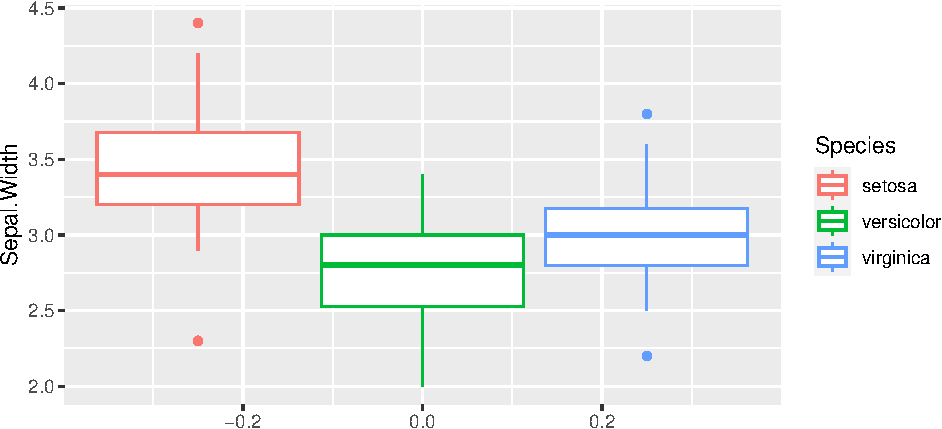
\includegraphics{paper_files/figure-latex/sample-fig1-1.pdf}
\caption{\label{fig:sample-fig1}This is a sample figure caption that
should interpret the figure!}
\end{figure}

Figure \ref{fig:sample-fig1} displays the side-by-side boxplots for
Sepal.Width by Species.

Figure \ref{fig:sample-fig2} displays a campus map.

\begin{figure}
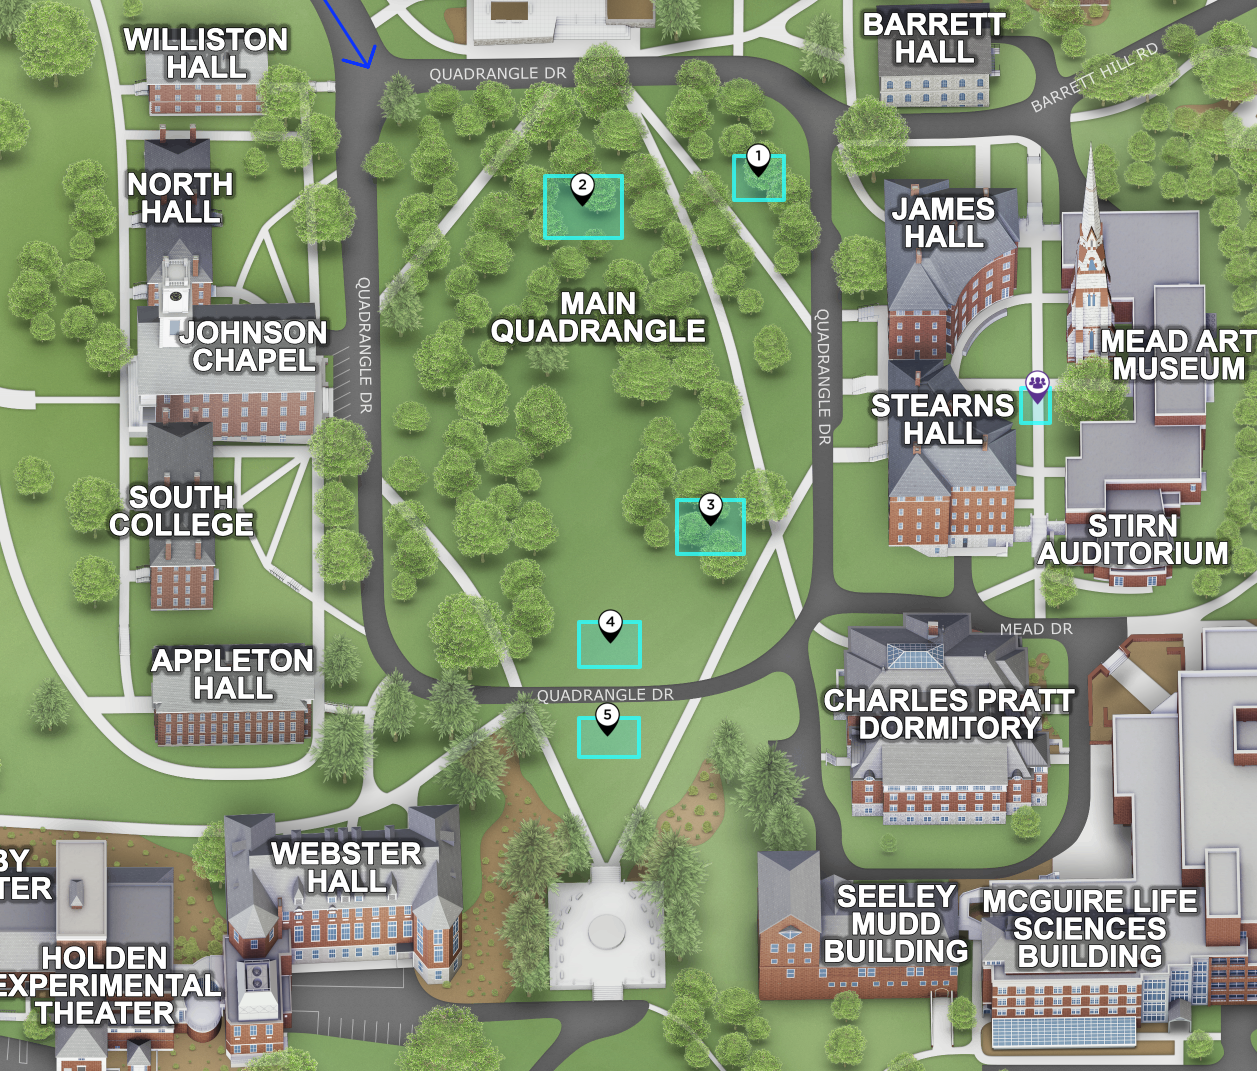
\includegraphics[width=0.8\linewidth]{gfx/campus_map} \caption{XX another sample figure caption}\label{fig:sample-fig2}
\end{figure}

\hypertarget{latex-examples}{%
\section{LaTeX Examples}\label{latex-examples}}

To shift into ``tex'' mode, it's pretty easy. You just need dollar
signs.

The variables \(X_1\) and \(X_2\) are uncorrelated.

If you have multiple indices or items that need to go into a subscript
or a superscript, you need curly brackets.

We want to look at \(X_{10}\) and \(X_{10}^{20}\).

If you have a big equation, you probably want to set it on it's own,
rather than try it in-line.

In regression, we assert (for two predictor variables) that

\[
\mu_Y = \beta_0 + \beta_1X_1 + \beta_2X_2.
\]

Don't forget punctuation in your equations.

If you want to reference equations, you need to be a bit more formal:

\begin{equation}
\label{regeq}
\mu_Y = \beta_0 + \beta_1X_1 + \beta_2X_2.
\end{equation}

Now I can refer to the equation as Equation \ref{regeq}.

I'm going to borrow a lot of the examples below from the revision of my
Probability textbook, so if the context is a little strange (meaning,
not from our class), that's why.

You can do bulleted lists using LaTeX instead of RMarkdown formatting
like this:

\begin{enumerate}
\item ``Define the terms: continuous RV, probability density function, and cumulative density function.
\item Compute expectation and variance for continuous RVs.
\item Apply uniform and exponential distributions to appropriate problems.
\item Solve problems involving joint and marginal distributions in the continuous setting.
\item Extend independence, covariance, and correlation concepts to the continuous setting.
\item Work with uniform and exponential distributions in R to find probabilities and simulate problems.'' (Chapter 6 introduction)
\end{enumerate}

In equations, you can also do alignments and adjust spacing with various
commands. In text, you can also get italics and bold text. Here is some
text with examples of these, including fractions in the equations.

``That is, we integrate a constant \(c\) over the bullseye region. This
leads to

\begin{align}
\label{pofb}
P(B) = \iint\limits_B c \, dx \, dy = c \left[  \mbox{Area}\,(B) \right] =  \frac{c \pi}{16}.
\end{align} What is \(c\)? As this is a probability model, the points in
the sample space should add up or integrate to 1. The sample space is
\(C\), the target. This gives

\[ 1 = P(C) = \iint\limits_{C} c \, dx \, dy =  c \left[ \mbox{Area}\,(C) \right] =c \pi\]

and thus \(c = 1/\pi.\) Plugging in \(c\) to Equation~\ref{pofb} gives

\[ P(B) = \frac{1}{\mbox{Area}\,(C)} \iint\limits_B \, dx \, dy = \frac{1}{16},\]

the proportion of the total area of the target taken up by the bullseye.

This gives the beginnings of a
\emph{continuous uniform probability model}. If \(\Omega\) is a
continuous set with all points equally likely, then for subsets
\(S \subseteq \Omega\),

\[ P(S) = \frac{1}{\mbox{Area}\,(\Omega)} \iint\limits_S \, dx \, dy = \frac{\mbox{Area}\,(S)}{\mbox{Area}\,(\Omega)}.\]

In one dimension, the double integral becomes a single integral and area
becomes length. In three dimensions we have a triple integral and
volume. (Chapter 6 introduction)'\,'

Here is an example from Chapter 6 with an alignment actually needed for
the two lines (the equals sign lines up):

\begin{align*}
1 & = \int_{-\infty}^{\infty} ce^{-|x|} \, dx   = \int_{-\infty}^0 c e^x \, dx + \int_0^{\infty} c e^{-x} \, dx \\
&= 2c \int_0^{\infty}  e^{-x} \, dx = 2c \left. (- e^{-x}) \right|_0^{\infty} = 2c,
\end{align*}

Here is an example from Chapter 6 with an array (for alignment) and text
inserted into the equation using mbox.

A random variable \(X\) has density function

\[ f(x) = \left\{ \begin{array}{@{}ll@{}}
2/5, & \mbox{ if } 0 < x \leq 1 \\[1ex]
2x/5, & \mbox{ if } 1 \leq x < 2 \\[1ex]
0, & \mbox{ otherwise.}  \end{array} \right.
\]

I think most of you will use kable or gtsummary for generating tables,
but if you want to make tables in LaTeX, you can do that too. Ask me for
assistance if you want to do that - I'm not including examples here.
Tables are MUCH easier to do in R using existing packages, imo, so I
would recommend that over LaTeX anyway.

\hypertarget{your-choice-of-structure}{%
\section{Your Choice of Structure}\label{your-choice-of-structure}}

You are responsible for choosing the structure you want for the report,
i.e.~what sections and their names. Here are some examples that you
could adapt, as appropriate. These are just examples - the first has
more sections, some of which may make more sense as sub-sections of
others. I'm just trying to give you examples. You don't have to have a
conclusion or an introduction, etc. You'll need to find what works for
you.

\hypertarget{example-1}{%
\subsection{Example 1}\label{example-1}}

\begin{itemize}
\tightlist
\item
  Introduction
\item
  Background
\item
  Topic X (Main exposition section)
\item
  Applications in Literature
\item
  Application to Data (your data)
\item
  Conclusion
\end{itemize}

\hypertarget{example-2}{%
\subsection{Example 2}\label{example-2}}

\begin{itemize}
\tightlist
\item
  Introduction (including any relevant Background)
\item
  Topic X (exposition and examples)
\item
  Simulation Study
\end{itemize}

\bibliographystyle{plainnat}
\bibliography{bibliography.bib}



\end{document}
